\begin{center}
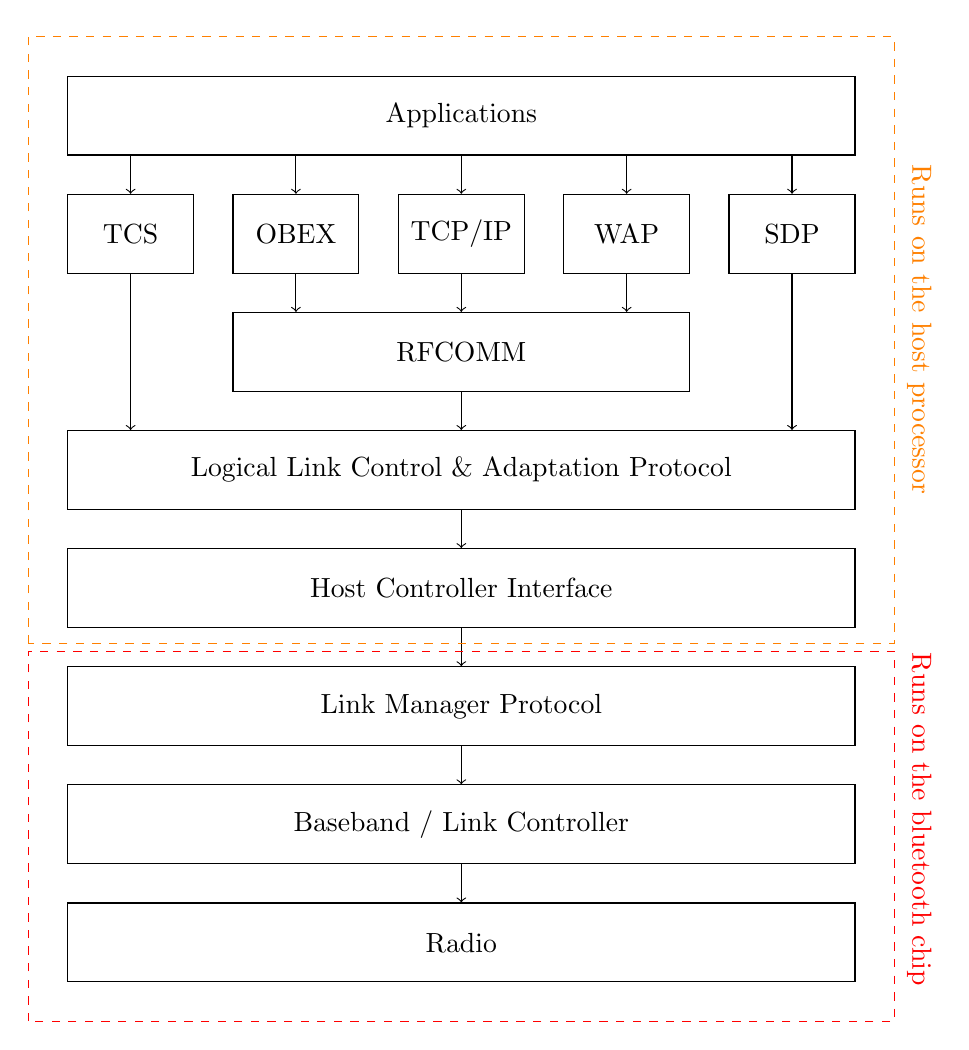
\begin{tikzpicture}

\node (A) at (5,-1) [draw,minimum width=10cm,minimum height=1cm] {Radio};
\node (B) at (5,0.5) [draw,minimum width=10cm,minimum height=1cm] {Baseband / Link Controller};
\node (C) at (5,2) [draw,minimum width=10cm,minimum height=1cm] {Link Manager Protocol};
\node (D) at (5,3.5) [draw,minimum width=10cm,minimum height=1cm] {Host Controller Interface};
\node (E) at (5,5) [draw,minimum width=10cm,minimum height=1cm] {Logical Link Control \& Adaptation Protocol};
\node (F) at (5,6.5) [draw,minimum width=5.8cm,minimum height=1cm] {RFCOMM};
\node (G1) at (0.8,8) [draw,minimum width=1.6cm,minimum height=1cm] {TCS};
\node (G2) at (2.9,8) [draw,minimum width=1.6cm,minimum height=1cm] {OBEX};
\node (G3) at (5,8) [draw,minimum width=1.6cm,minimum height=1cm] {TCP/IP};
\node (G4) at (7.1,8) [draw,minimum width=1.6cm,minimum height=1cm] {WAP};
\node (G5) at (9.2,8) [draw,minimum width=1.6cm,minimum height=1cm] {SDP};
\node (H) at (5, 9.5) [draw,minimum width=10cm,minimum height=1cm] {Applications};

\draw [->] (G1 |- H.south) -- (G1);
\draw [->] (G2 |- H.south) -- (G2);
\draw [->] (G3 |- H.south) -- (G3);
\draw [->] (G4 |- H.south) -- (G4);
\draw [->] (G5 |- H.south) -- (G5);
\draw [->] (G1.south) -- (G1 |- E.north);
\draw [->] (G2.south) -- (G2 |- F.north);
\draw [->] (G3.south) -- (G3 |- F.north);
\draw [->] (G4.south) -- (G4 |- F.north);
\draw [->] (G5.south) -- (G5 |- E.north);
\draw [->] (F) -- (E);
\draw [->] (E) -- (D);
\draw [->] (D) -- (C);
\draw [->] (C) -- (B);
\draw [->] (B) -- (A);

\draw [dashed, orange] (-0.5, 2.8) rectangle (10.5, 10.5) node [label={[label distance=1.5cm,text depth=3ex,rotate=-90, orange]right:Runs on the host processor}] {};
\draw [dashed, red] (-0.5, -2) rectangle (10.5, 2.7) node [label={[label distance=-0.1cm,text depth=3ex,rotate=-90, red]right:Runs on the bluetooth chip}] {};

\end{tikzpicture}
\captionof{figure}{Classic Bluetooth protocol stack}
\end{center}